\section{Interference Differential Cross Sections}
Because the ion-ion elastic scattering collisions consist of two parts (Coulomb and NES), a quantum mechanical interference differential cross section appears that describes the mutual interference between the two types of elastic scattering collisions \cite{Devaney-1971}. Therefore, the total elastic scattering differential cross section is written as
\begin{equation}
    \sigma_{x,t \rightarrow x} = \sigma_{x,t \rightarrow x}^C + \sigma_{x,t \rightarrow x}^N + \sigma_{x,t \rightarrow x}^I,
\end{equation}
where the superscripts $C$, $N$, and $I$ represent the Coulomb, NES, and interference components of the total ion-ion elastic scattering differential cross section. The differential cross sections that describe Coulomb collisions have an analytical form; while the differential cross sections that describe the NES, interference, and nuclear reactions collisions are tabulated in data sets. The remainder of this section presents the analytical form of the Coulomb differential cross section, and the forms of the tabulated differential cross sections describing the NES, interference, and nuclear-reaction collisions.

In Figure \ref{fig:sig_i}, the interference differential cross section for energetic deuterons colliding with tritons is shown for various incident energies. Looking at Figure \ref{fig:sig_i}, as $\mucm \rightarrow 1$ the interference differential cross section oscillates between positive and negative values of increasing magnitude. Negative differential cross sections have no physical meaning, and therefore the interference differential cross section must be combined some other differential cross section such that the resulting differential cross section is always positive.

\begin{figure}[!htb]
    \centering
    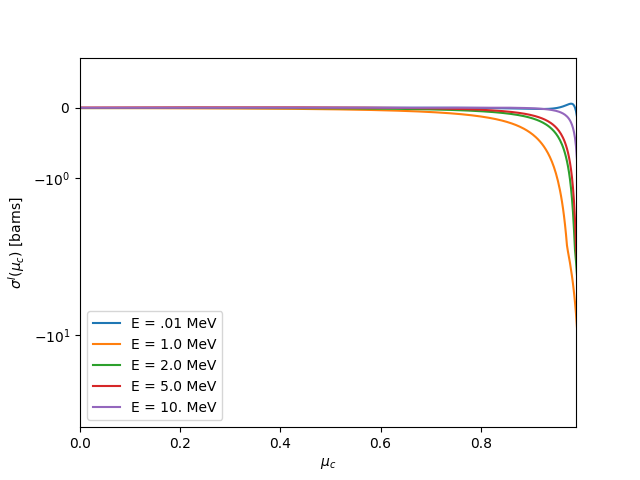
\includegraphics[scale=0.75]{../figures/proposed_work/sig_i_dt.png}
    \caption{Interference scattering differential cross section for deuterons colliding with tritons at 1.0 MeV}
    \label{fig:sig_i}
\end{figure}